\chapter{Cronograma}
\label{cap:cronograma}

A Figura \ref{fig:cronograma} ilustra o planejamento integral desta pesquisa de mestrado ao
longo de um período de 24 meses, detalhando a sequência e a duração das principais fases e
atividades. A primeira fase, denominada Fundamentação e Planejamento, é visualizada abrangendo
aproximadamente os sete meses iniciais do projeto. Esta etapa compreende atividades essenciais
como o cumprimento dos créditos disciplinares do programa (representado por uma barra
estendendo-se dos meses 1 a 10, indicando sobreposição com atividades subsequentes), o
levantamento bibliográfico inicial e a definição precisa do tema de pesquisa (meses 1--3), a
elaboração da primeira versão do projeto de pesquisa, e um período de aprofundamento nos
fundamentos teóricos sobre identidade de lugar, percepção de lugar, e nas metodologias centrais
como Design Science, Processamento de Linguagem Natural (NLP) e análise de sentimento (meses
4--7).

A segunda fase, Revisão Sistemática e Desenvolvimento Metodológico e Ferramental, é
representada no gráfico estendendo-se aproximadamente do sexto ao décimo quarto mês. As barras
indicam a condução da Revisão Sistemática da Literatura (\gls{RSL}) sobre análise de sentimento
aplicada (meses 6--9), uma etapa já consolidada conforme detalhado neste documento. Segue-se o
estudo e a seleção de ferramentas para análise de sentimento, que incluiu testes preliminares com
diversas APIs e culminou na escolha da API Gemini (meses 9--12), cujos resultados parciais
justificam a seleção. Em paralelo e subsequentemente, ocorre o desenvolvimento ou adaptação da
plataforma Gnomon para otimizar a coleta de dados textuais específicos para os objetivos da
pesquisa (meses 10--14). A elaboração deste documento de Qualificação encerra esta fase,
visualizada entre os meses 12 e 14.

\begin{figure}[h]
    \centering
    \caption{Cronograma de Atividades}
    \label{fig:cronograma}
    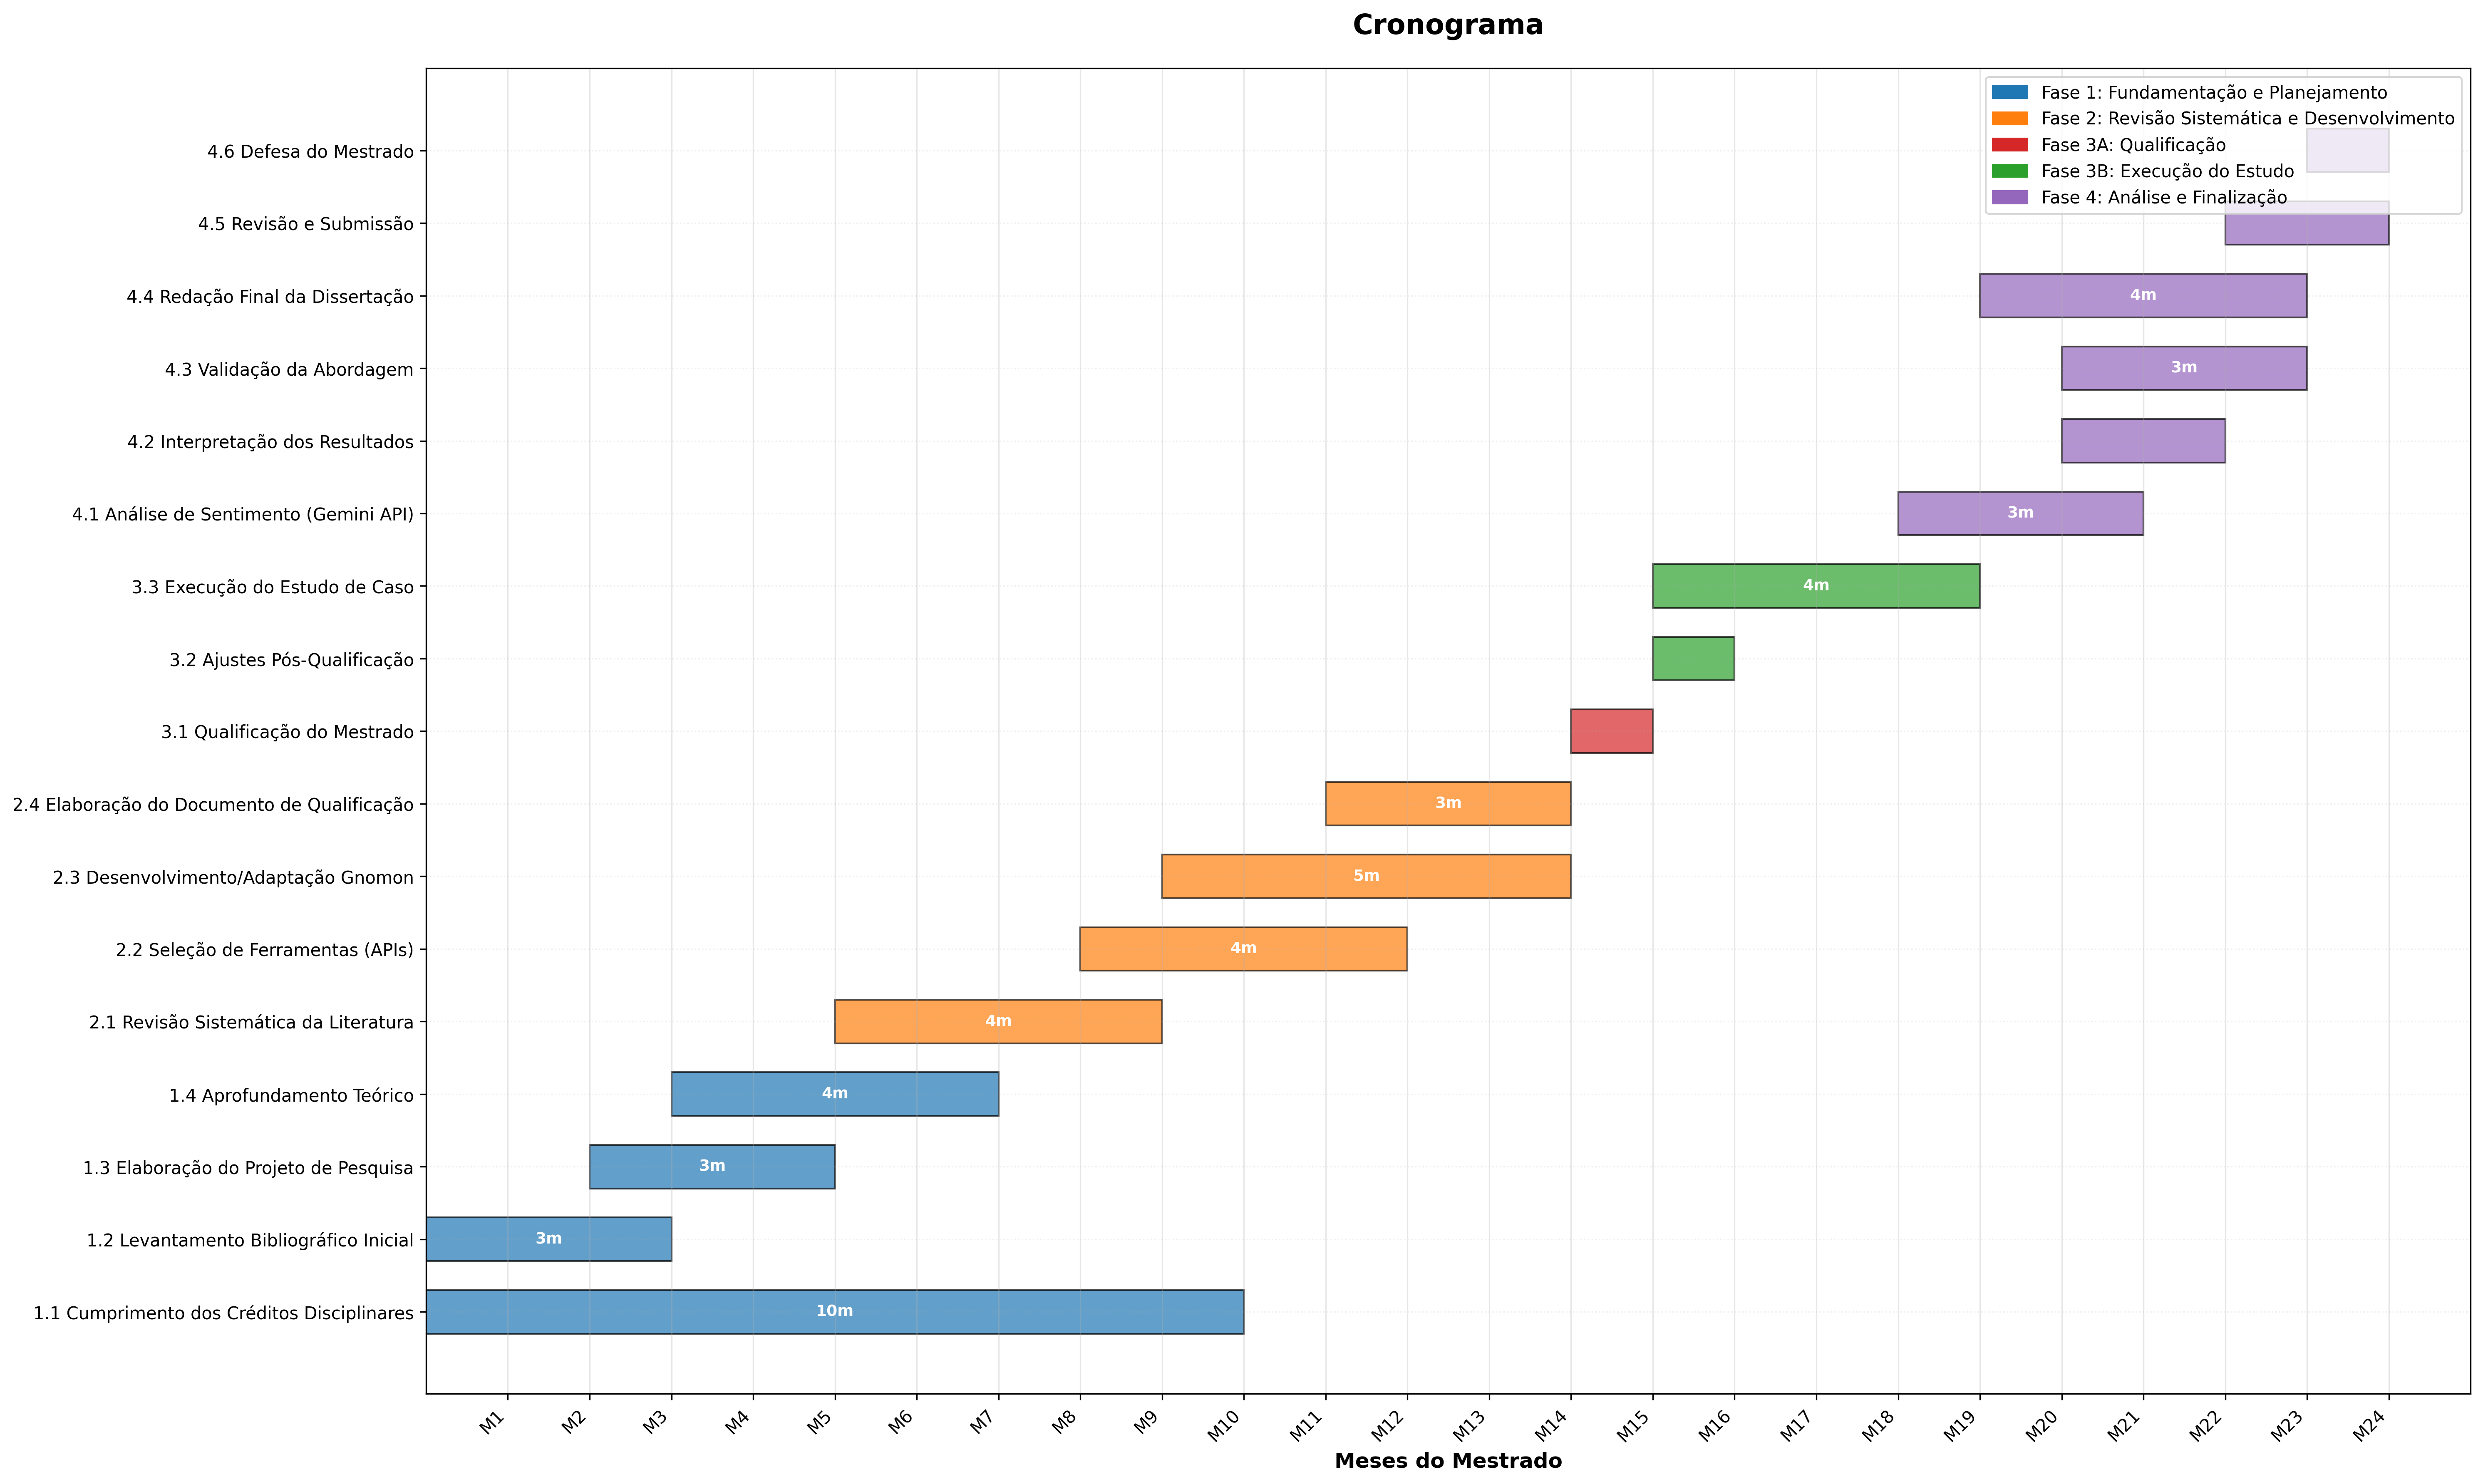
\includegraphics[width=\textwidth]{figuras/cronograma}
    \legend{Fonte: Autoria Própria (2025).}
\end{figure}

A terceira fase, Qualificação e Execução do Estudo de Caso, tem um marco central no Mês
15, destacado no gráfico como o período da Qualificação do Mestrado, momento atual da pesquisa.
Imediatamente após, no Mês 16, os ajustes na proposta de pesquisa, incorporando as contribuições
da banca examinadora. A etapa subsequente, crucial para a coleta de dados primários, é a execução
do estudo de caso com a plataforma Gnomon, envolvendo a interação efetiva de usuários e a
geração de dados textuais, representada por uma barra que se estende dos meses 16 ao 19.

Finalmente, a quarta fase, Análise de Dados, Redação Final e Defesa, ocupa os meses 19 a
24 do cronograma. O gráfico detalha o processamento e a análise de sentimento dos dados
coletados utilizando a API Gemini (meses 19--21), seguida pela interpretação dos resultados
focada na percepção de lugar e identidade territorial, e a discussão destes à luz do referencial
teórico (meses 21--22). A validação da abordagem metodológica e dos resultados, conforme os
princípios da Design Science, está prevista para os meses 21 a 23. A redação final da dissertação é
representada como uma atividade contínua que se sobrepõe a estas etapas analíticas (meses
20--23). Concluindo o cronograma, a revisão e submissão da dissertação ocorrem entre o Mês 23 e
o início do Mês 24, com a preparação para a defesa e a defesa do mestrado programadas para o
final do Mês 24, encerrando o ciclo da pesquisa.
